To set up the AMC13, it must be installed in the upper slot 13 of the $\mu$TCA crate, with the MCH in the lower slot, as shown in Fig.~\ref{fig:amc13}. All communication with the AMC13 is performed via the network connection on the MCH. Data is read out of the AMC13 via a 10 Gb fiber that should be connected to the top (DAQ0) SFP+ port on the AMC13. 

\begin{figure}
\centering
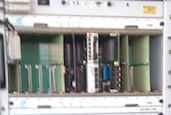
\includegraphics{figs/amc13.png}
\label{fig:amc13}
\caption{An AMC13 in a $\mu$TCA crate.}
\end{figure}

For general use, all configuration of the AMC13 should be handled automatically by the DAQ code. For expert users, it may be necessary to configure and run the AMC13 manually using the program amc13tool2.exe, which is provided in the gm2daq repository. 